\documentclass[10pt]{article}
\usepackage{lingmacros}
\usepackage{graphicx}
\usepackage{caption}
\usepackage{subcaption}
\usepackage{amsmath}
\usepackage[margin=0.75in]{geometry}


\begin{document}

\title{Symbols, Patterns \& Signals - CW2: A Memory of Wine}
\author{Saif Anwar \& Tommy Van Aalst}
\date{}
\maketitle


\section*{Introduction}
\section*{Choosing the best features}

To choose the best features we observed all the plots of the pairwise combinations of the features and tried to find the ones which separated the data points into the three classes the best.
There are some which clearly do not work, because the data points are overlapping and there is clearly no way to separate them into their three classes.

\begin{figure}[h!]
\captionsetup[subfigure]{labelformat=empty}
\begin{subfigure}{.5\textwidth}
\centering
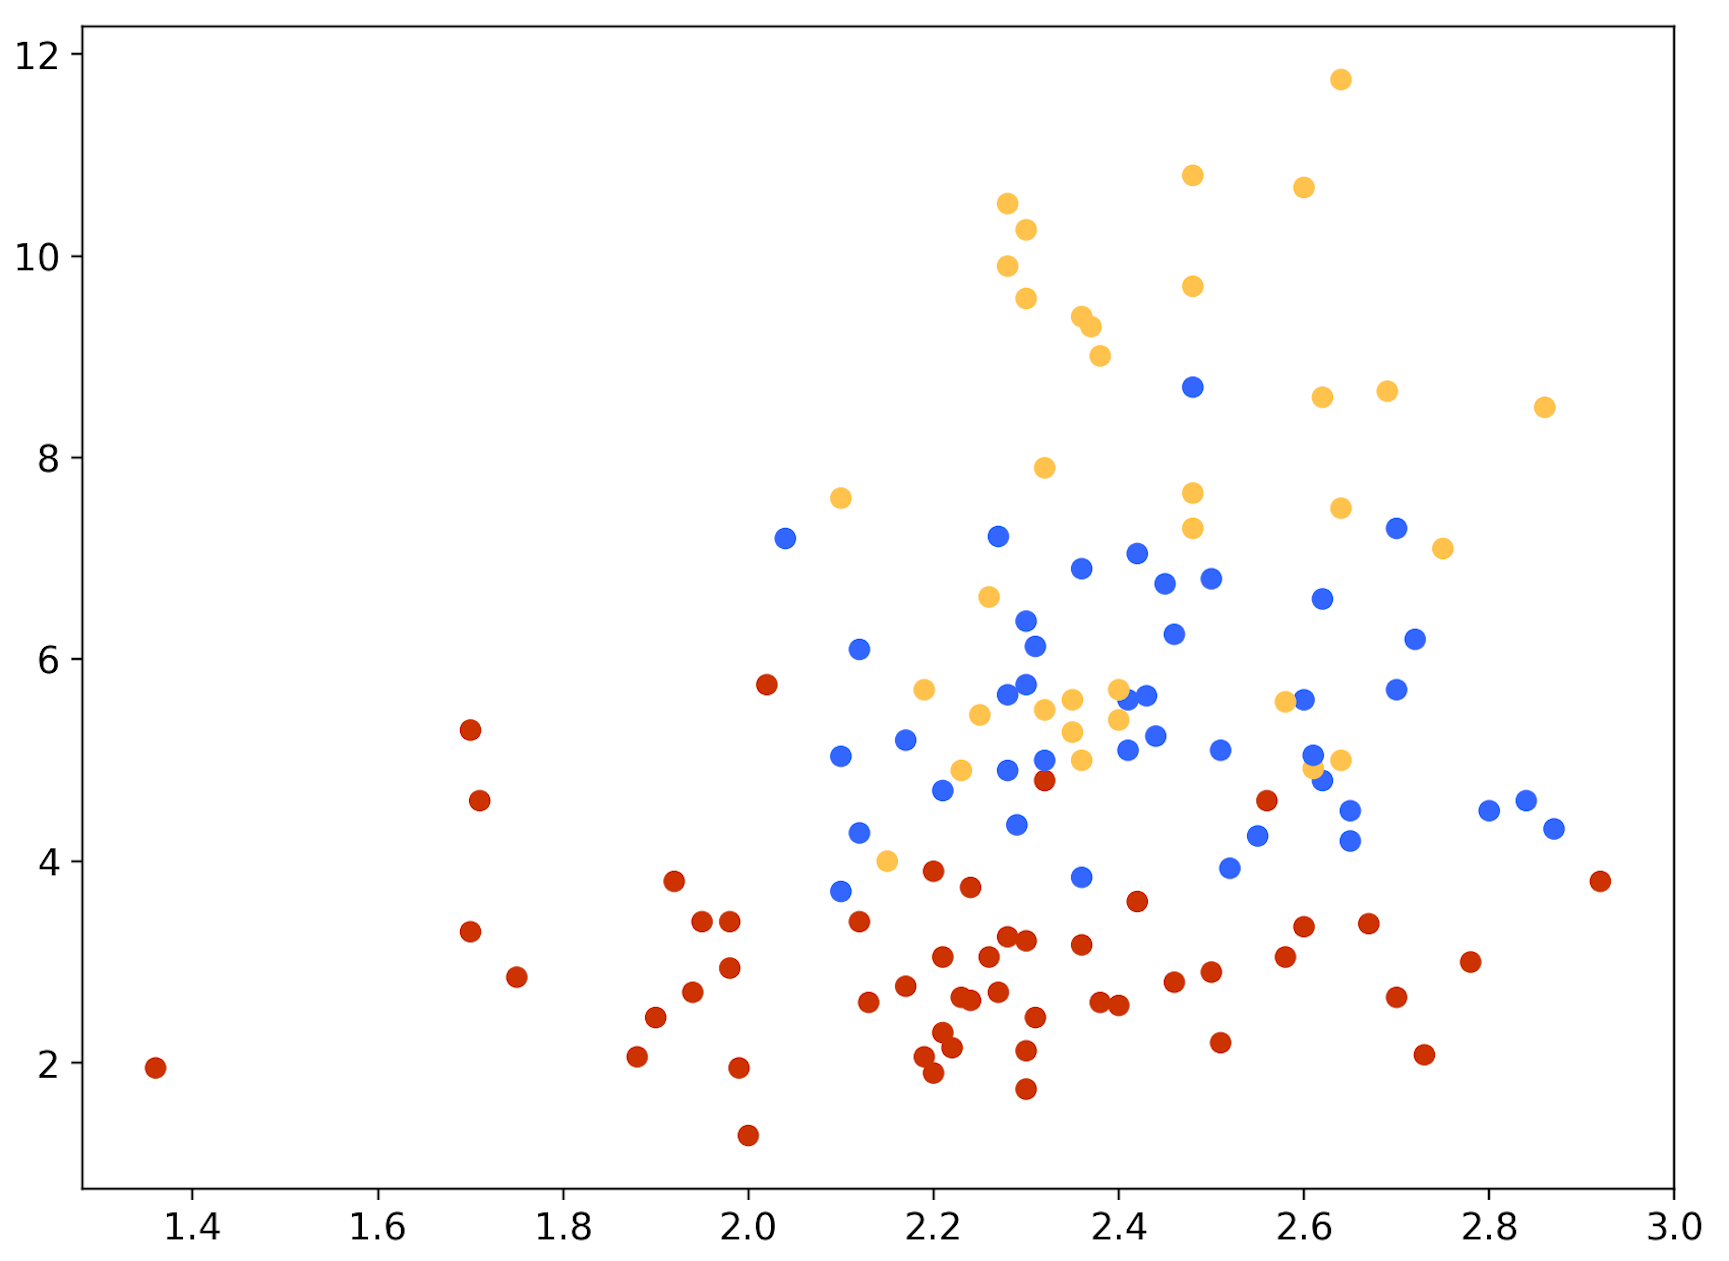
\includegraphics[height=4.2cm]{3and10.png}
\caption{Fig 1: Plot of features 3 and 10}
\end{subfigure}%
\begin{subfigure}{.5\textwidth}
\centering
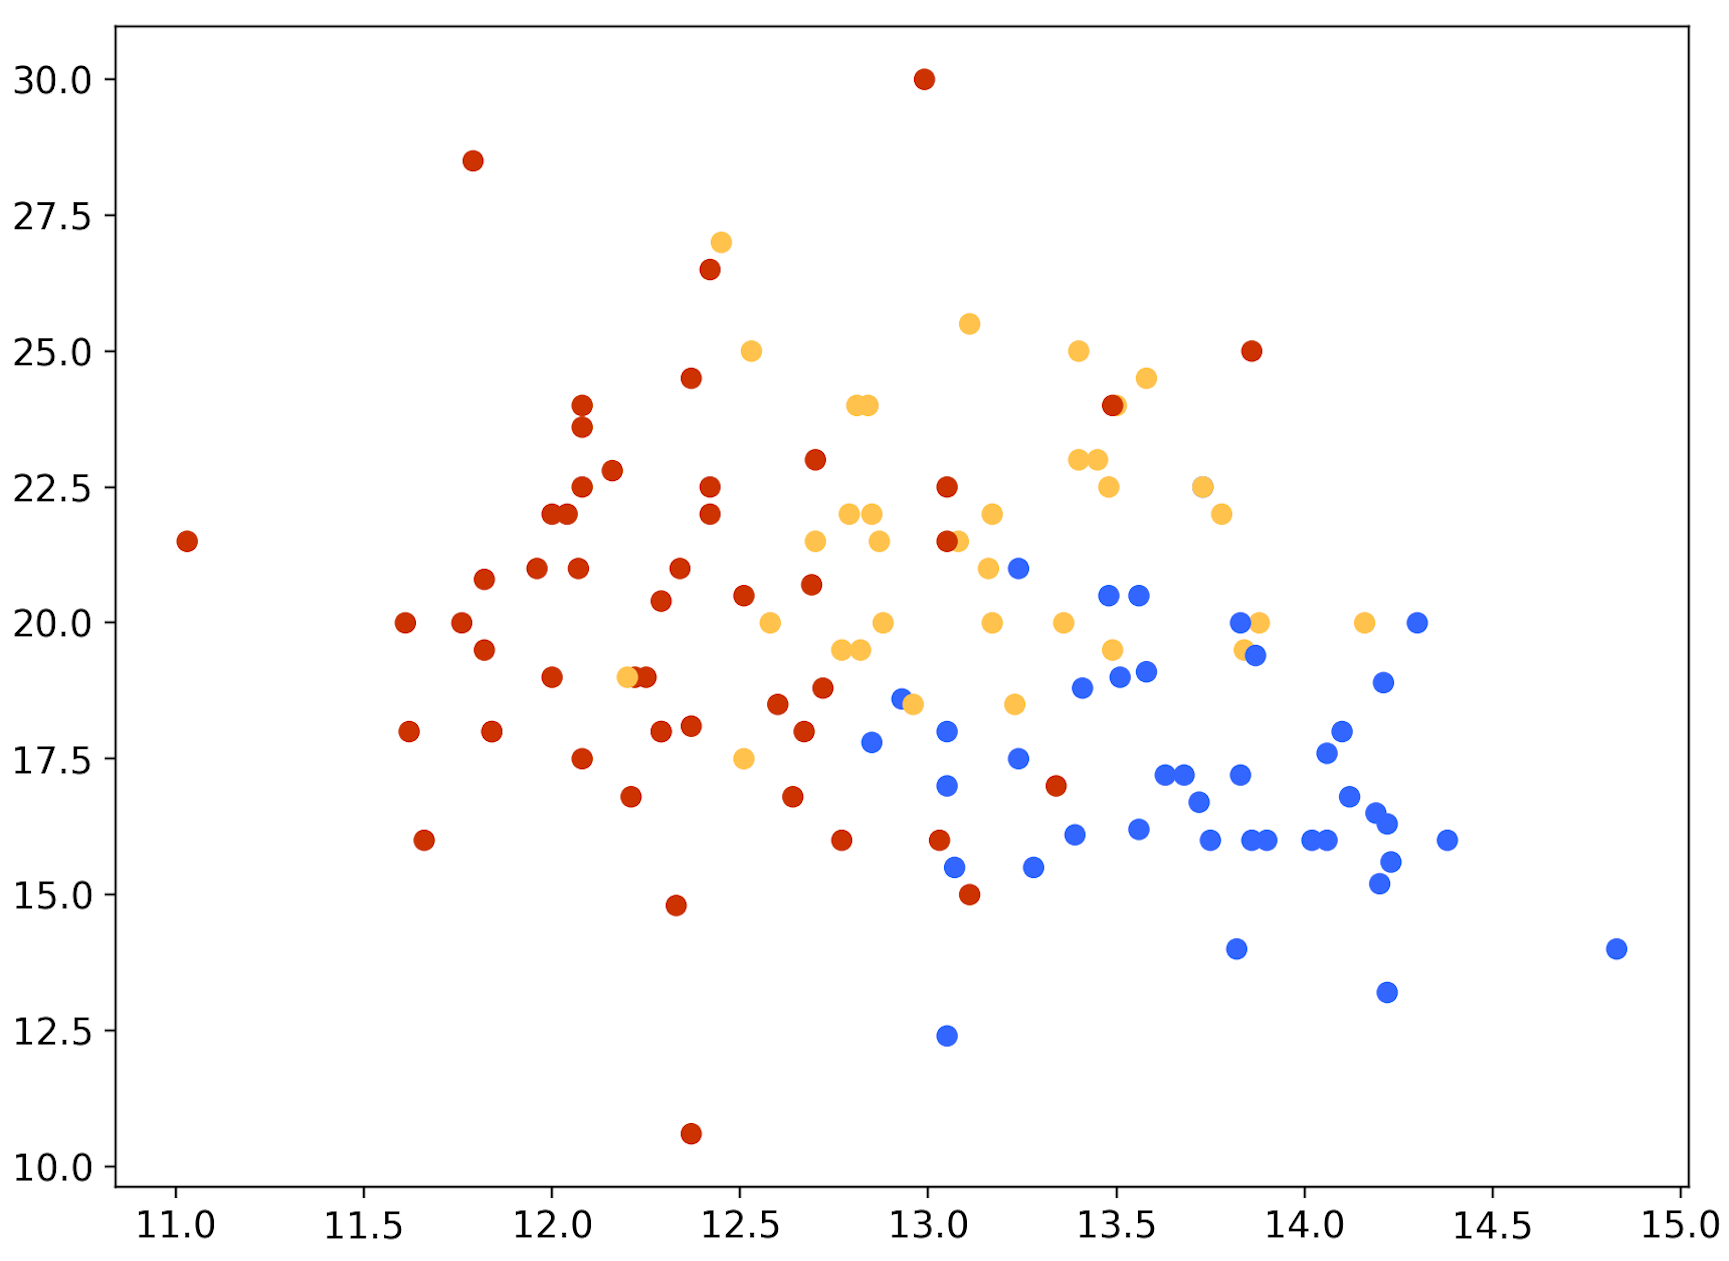
\includegraphics[height=4.2cm]{1and4.png}
\caption{Fig 2: Plot of features 1 and 4}
\end{subfigure}%
\end{figure}
\noindent
Here you can see in Fig 1 that although the red class is somewhat separable from the other two, the blue and yellow completely mix. It would be impossible to separate them in any way. In Fig 2 each class is in its own part of the plot, however in the middle they all overlap, again meaning there is no way to clearly separate the points into their three classes.\\

\noindent
There are also a quite a few which do all work well, like these ones below:

\begin{figure}[h!]
\captionsetup[subfigure]{labelformat=empty}
\begin{subfigure}{.5\textwidth}
\centering
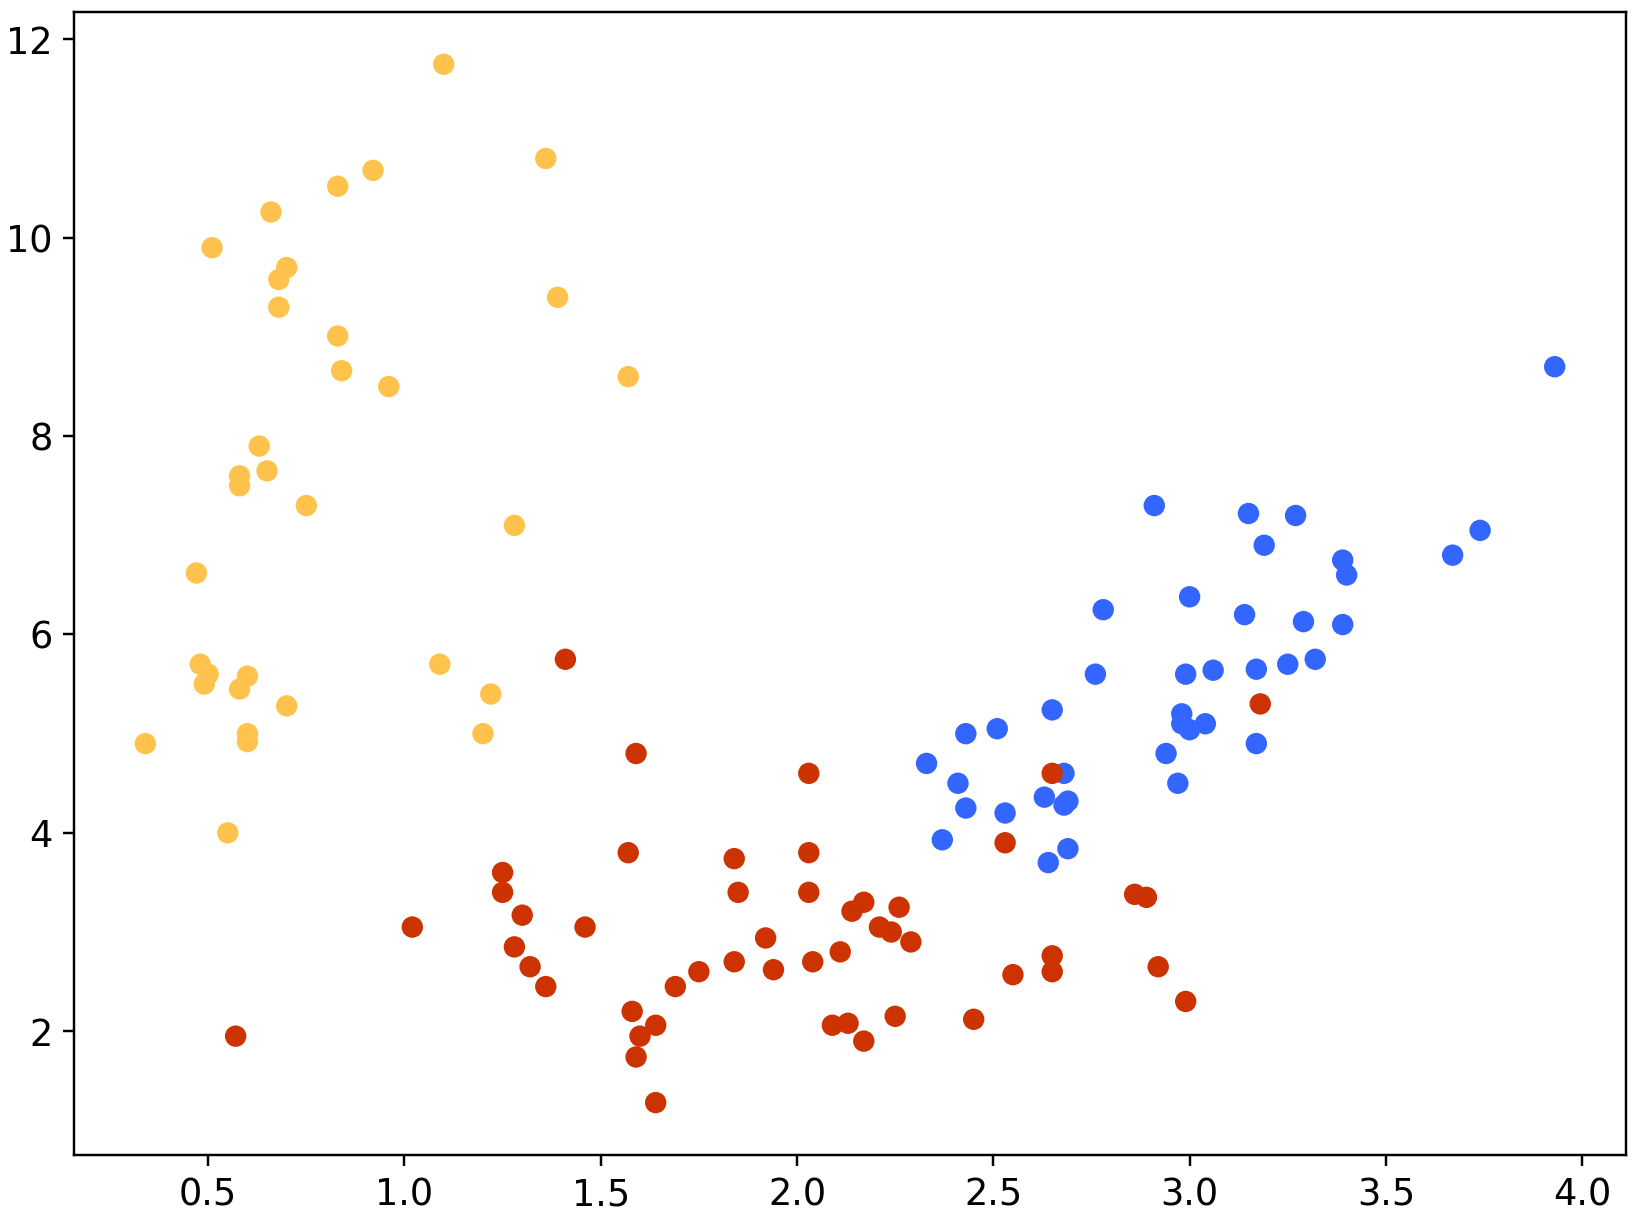
\includegraphics[height=4.2cm]{7and10.png}
\caption{Fig 3: Plot of features 7 and 10}
\end{subfigure}%
\begin{subfigure}{.5\textwidth}
\centering
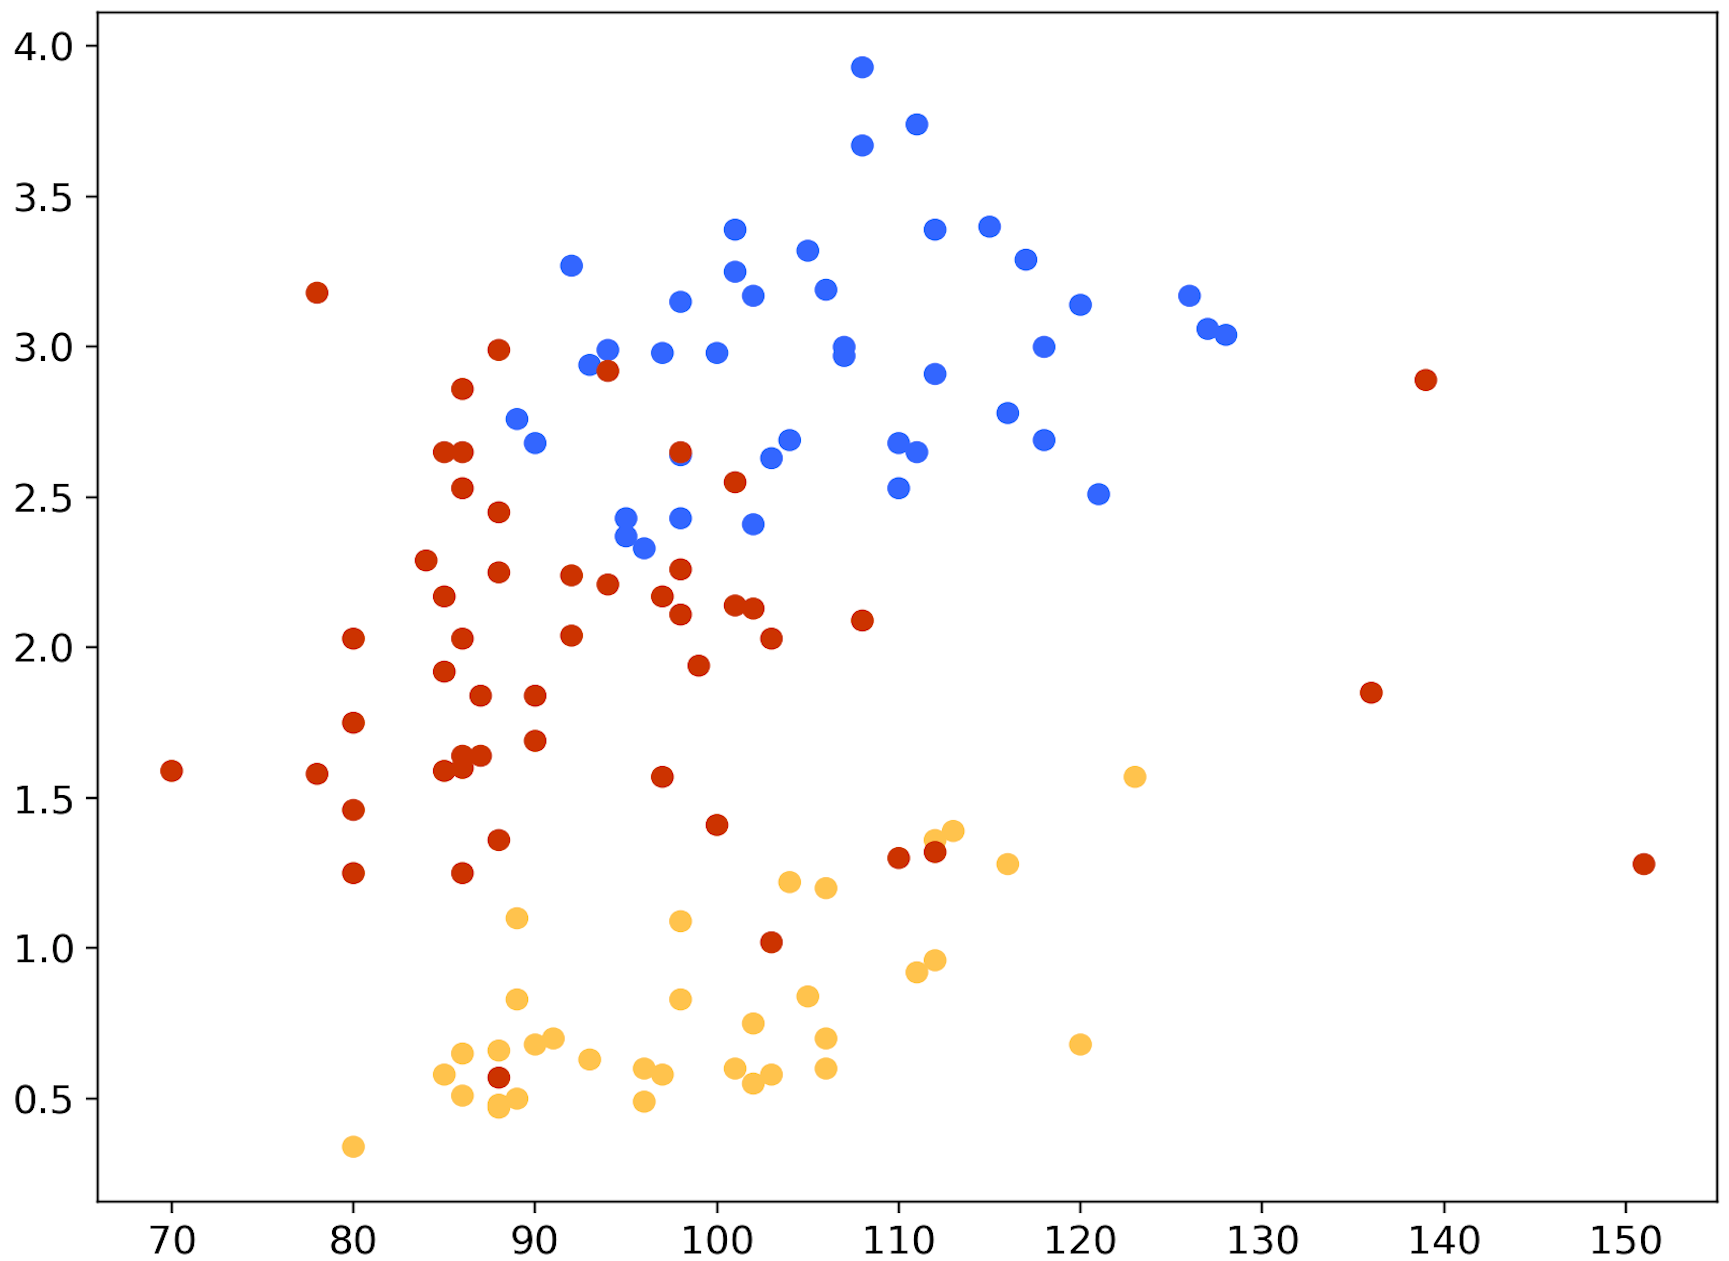
\includegraphics[height=4.2cm]{5and7.png}
\caption{Fig 4: Plot of features 5 and 7}
\end{subfigure}%
\end{figure}
\noindent
\\
\noindent
Here you can see clearly in Fig 3 that you can separate each of the classes well. There is some slight overlap on the edges but not much. Also, each class only has a boundary to one other class. All three classes don’t overlap together in the middle so the boundary data could be only one of two classes, not one of three, therefore resulting in more accurate predictions. Fig 4 is quite good however there is a little bit of overlap between the blue and red classes and the red class has some outliers spread out. We concluded to choose features 7 and 10.\\

\noindent
We also ran a script to calculate the accuracies of each pairwise combination. We found that the features we chose gave relatively good accuracy in each of our classifiers.

\section*{K-Nearest Neighbours}

We implemented the K-Nearest Neighbours (knn) algorithm using functions to represent the steps. The first step is to calculate the Euclidean Distance between the wine in question from the wine\_test set and every wine from the wine\_train set. For a two-dimensional knn this will only be for the two selected features using the following formula:
$$d(x,y) = \sqrt{\sum_{n=1}^{k} (x_i - y_i)}$$
\\
\noindent
From all of these distances we can now find the k smallest distances to get the nearest neighbours when the test wine is plotted onto the scatter of the train sets selected features.\\

\noindent
Now we have to assign a class to each of the neighbours by reading the wine\_train\_labels file to get an idea of what classes are closest to our test wine graphically. From this we can assume and assign a class to our test wine. Depending on the selected number of nearest neighbours, k, we may or may not have a modal class amongst our neighbours. If k=1 then we have an obvious mode of the single class and our test wine can be assumed to be of this class. Any k higher than this invites the possibility for multiple mode classes in the nearest neighbours. In this situation we recalculate the modal classes for k-1 neighbours which eliminates the furthest neighbour. This is repeated until we successfully find a mode which is then assigned as our test wines class.\\

\noindent
We can repeat this process for each of the wines in the wine\_test set and create our list of predictions for the test set. By comparing our predictions with the provided wine\_test\_labels, we can calculate an accuracy for our algorithm using the following formula:
$$Accuracy = \frac{\text{Number of Correctly Predicted Wines}}{\text{Total Number of Wines}}$$
\\
\noindent
We observed that for our selected features (1 and 7) we would get a reasonably high accuracy of 88.68\%. As the number of nearest neighbours is increased, a higher accuracy is expected as it reduces the potential of plots from the train set that have anomalous positions on the scatter plot to affect the classification of the the test wine. Picking numerous neighbours will give a better overall prediction of the class. This can be observed from the general increase in accuracy as the number of neighbours is increased. The effect is drastic when observed in the situation where we select 5 neighbours, still using the features 1 and 7, the accuracy of the classifier becomes 100\%. This can cause implications however as we do not want the classifier to overfit to the training data. To avoid overfitting, the training set size can be increased.\\

\noindent
Here are the confusion matrices for each of the values of $k \in (1,2,3,4,5,6,7)$

$$
k=1,2
\begin{bmatrix} 
0.78 & 0.22 & 0\\
0 & 1 & 0\\
0 & 0.14 & 0.86
\end{bmatrix}
\quad
k=3,4
\begin{bmatrix} 
0.94 & 0.06 & 0\\
0 & 1 & 0\\
0 & 0.14 & 0.86
\end{bmatrix}
\quad
k=5, 6, 7
\begin{bmatrix} 
1 & 0 & 0\\
0 & 1 & 0\\
0 & 0 & 1
\end{bmatrix}
\quad
$$
\\
\noindent
It can be observed that there are no wrong predictions between 1 and 3 (1 being classed as three and vice versa). This was expected as there is not an approximate boundary, in the scatter plot of the features, that is shared by both classes 1 and 3. From k=5 onwards, it can be seen that all the values along the diagonal's are 1 which indicates 100\% accuracy of the classifier as there are no incorrectly classified wines.

\section*{Alternate Classifier - Na\"ive Bayes Classifier}
-\\
-\\
-\\





\section*{K-Nearest Neighbours with three features}

Constructing the KNN Classifier with 3 features adds a new dimension to calculating the Euclidean Distance between the points. It incorporates all the possible combinations of the three features. For example, we selected features 1,2 and 7; proceeded to plot them on a 3-dimensional axis to observe the boundaries between the classes. Observing the 3d scatter plot perpendicular to each of the axis will give you the 2d plot of the other two features. Doing this in turn will give you an idea of the relationship between each of the features individually. \\

\noindent
Here are some plots of features 1,2 and 7 in 3d space from each axis:

\begin{figure}[h!]
\captionsetup[subfigure]{labelformat=empty}
\begin{subfigure}{.33\textwidth}
\centering
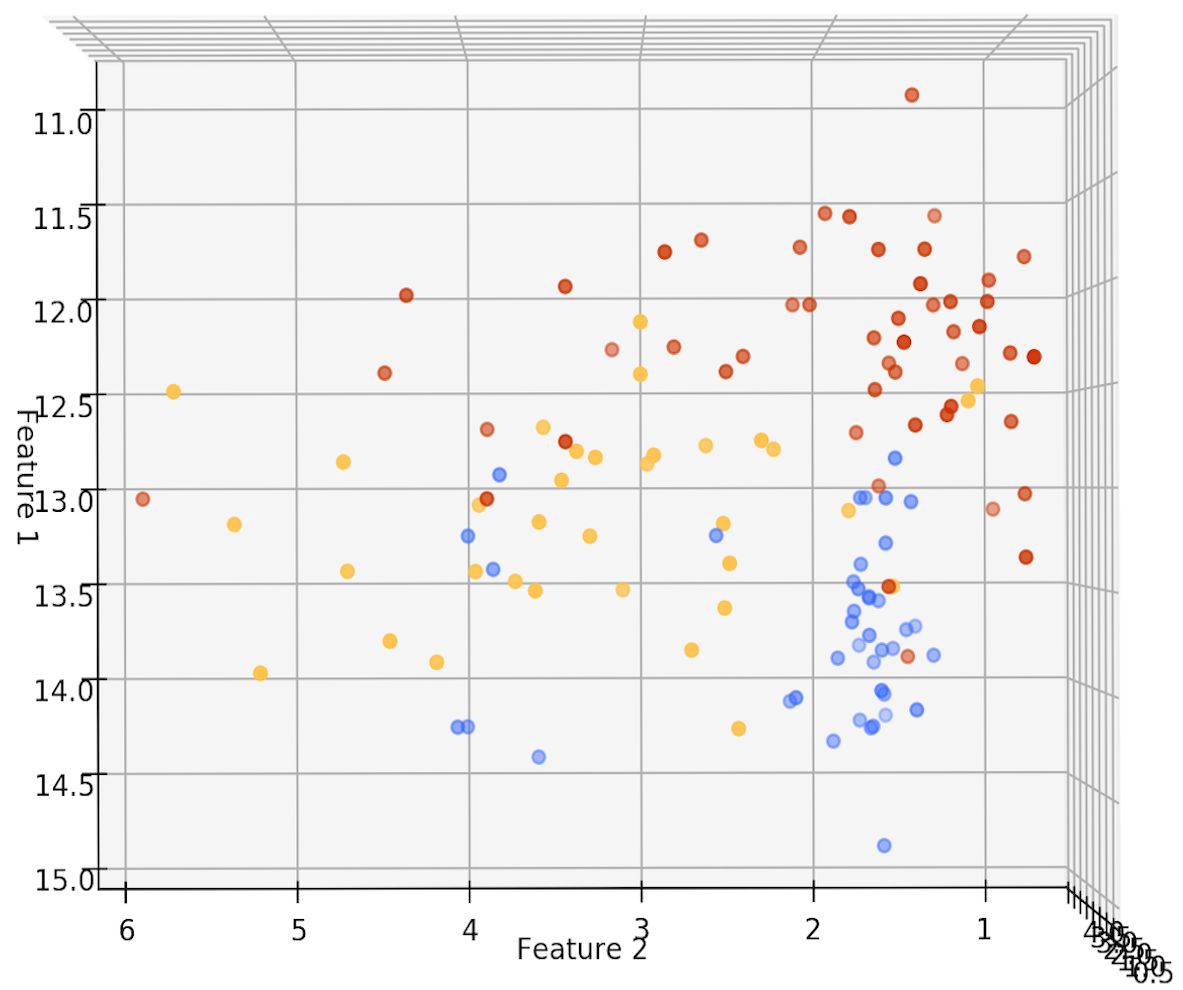
\includegraphics[height=4.2cm]{3d1x2.png}
\caption{Fig 5: Plot of features 1 and 2 in 3d space}
\end{subfigure}%
\begin{subfigure}{.33\textwidth}
\centering
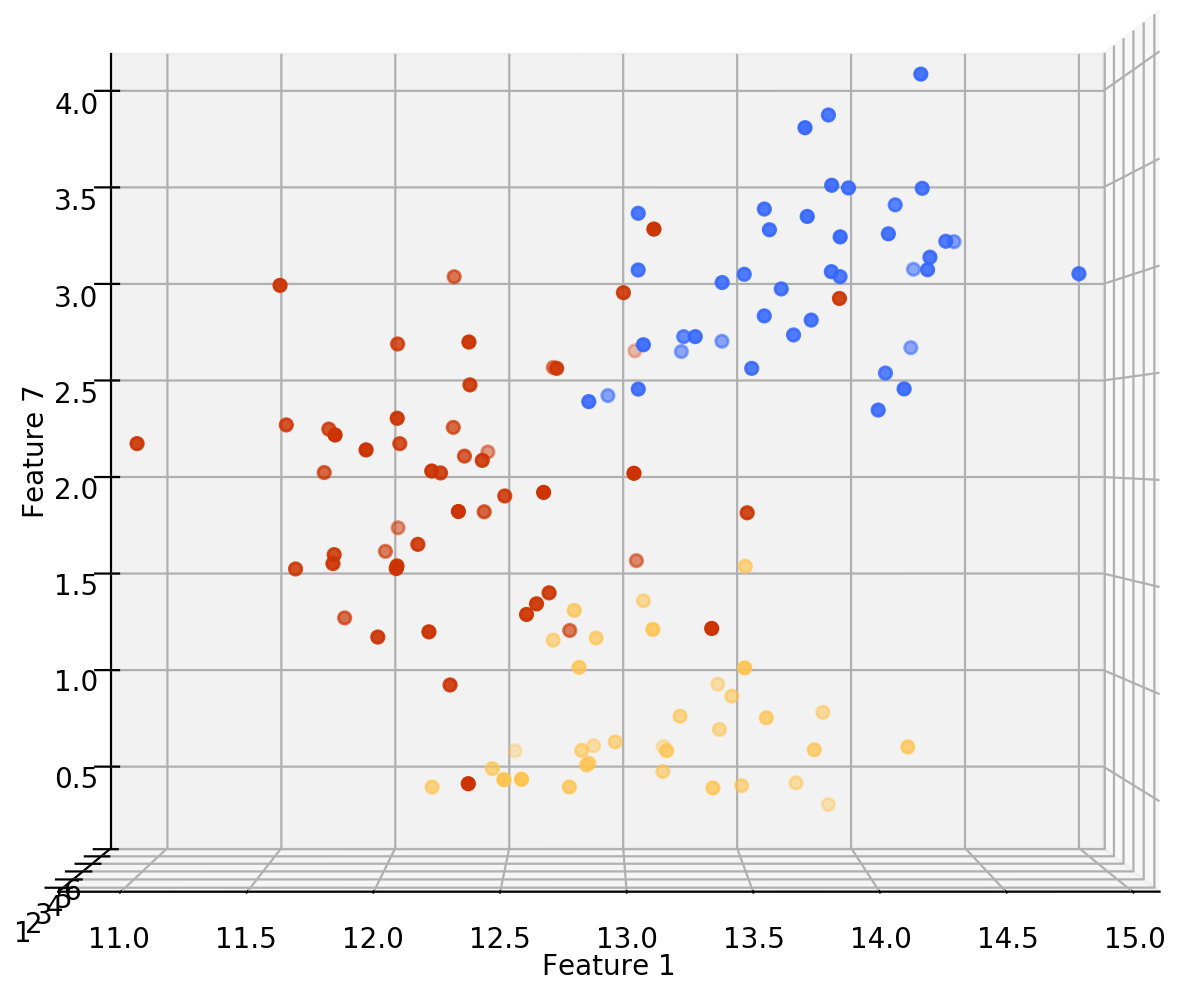
\includegraphics[height=4.2cm]{3d1x7.png}
\caption{Fig 6: Plot of features 1 and 7 in 3d space}
\end{subfigure}%
\begin{subfigure}{.33\textwidth}
\centering
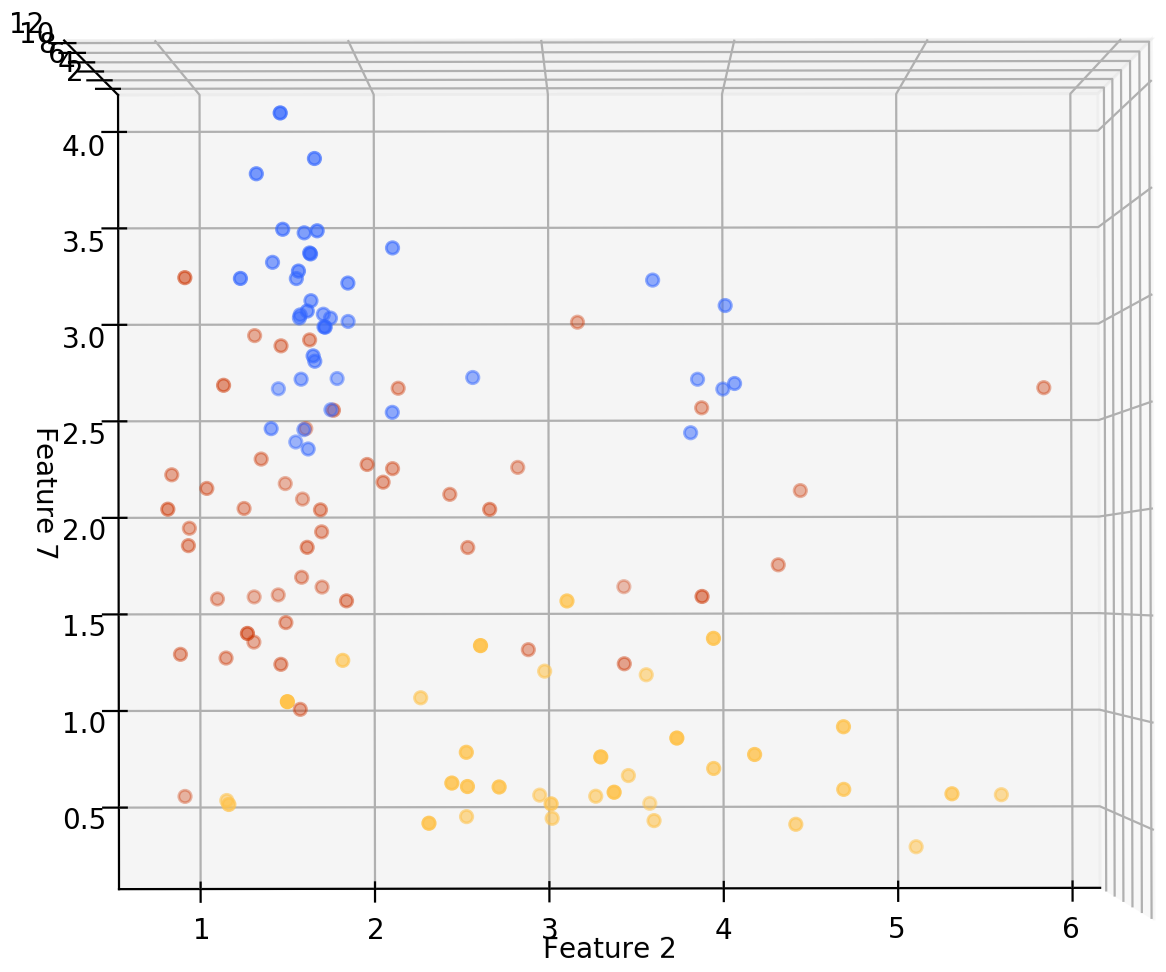
\includegraphics[height=4.2cm]{3d2x7.png}
\caption{Fig 7: Plot of features 2 and 7 in 3d space}
\end{subfigure}%
\end{figure}

\noindent
Using three features can either be beneficial by picking features that compliment each other in their individual plots against the other features, or can in fact make the classifier worse overall due to a single pair of the combinations not showing a strong distinctive relationship between the classes. To select our 3 features, we kept our 2 features from our original KNN classifier so we could see what difference a single new dimension would make without changing our other features. We used a script to calculate the accuracy from each selection and we deemed feature 2 to be a fitting addition to the KNN classifier.  As can be seen in the figures above, each of the pairwise combinations of features show reasonable boundaries between each of the classes confirming that (1,2,7) is a suitable set of features to use for our 3d KNN classifier. \\

\noindent
We can compare the accuracy between using 3 features and using 2 features by comparing the confusion matrices for $k \in (1,2,3,4,5,6,7)$:

$$
k=1,2,3,4
\begin{bmatrix} 
0.94 & 0.06 & 0\\
0 & 1 & 0\\
0 & 0.07 & 0.93
\end{bmatrix}
\quad
k=5,6,7
\begin{bmatrix} 
1 & 0 & 0\\
0 & 1 & 0\\
0 & 0.07 & 0.93
\end{bmatrix}
\quad
$$
\noindent
\\
\noindent
From the matrices for KNN3d we can see that for smaller values of $k \in(1,2,3,4)$ the accuracy is better than KNN with 2 features whereas for larger values of $k \in(5,6,7)$ the accuracy is not as good. This would be due to feature 2 either contributing in a way that improves the accuracy or contributes incorrectly, thus making our classifier worse. The plot of features 1 \& 2 shows multiple crossovers the classes and doesn’t show distinct boundaries. This would negatively affect our classifier when taking more neighbours into account. The only difference between the confusion matrices for all the values of k is there are instances for $k \in(1,2,3,4)$ where there are wines predicted as class 2 when they are actually of class 1. This can be seen to possibly be due to the pairwise combination of features 2 \& 7 where there is significant crossover between class 1 (Blue) and class 2 (Red).

\section*{K-Nearest Neighbours Using Principle Component Analysis (PCA)}
Principal Component Analysis (PCA) is a method to reduce the dimensionality of the data. It extracts the most useful parts of the data whilst aiming to maintain the same level of accuracy within the classifier. Using the PCA implementation from the Scipy library, we reduced our training data.\\

\noindent
The following is a scatter plot of the PCA-reduced data and the original scatter plot of the features we selected:

\begin{figure}[h!]
\captionsetup[subfigure]{labelformat=empty}
\begin{subfigure}{.5\textwidth}
\centering
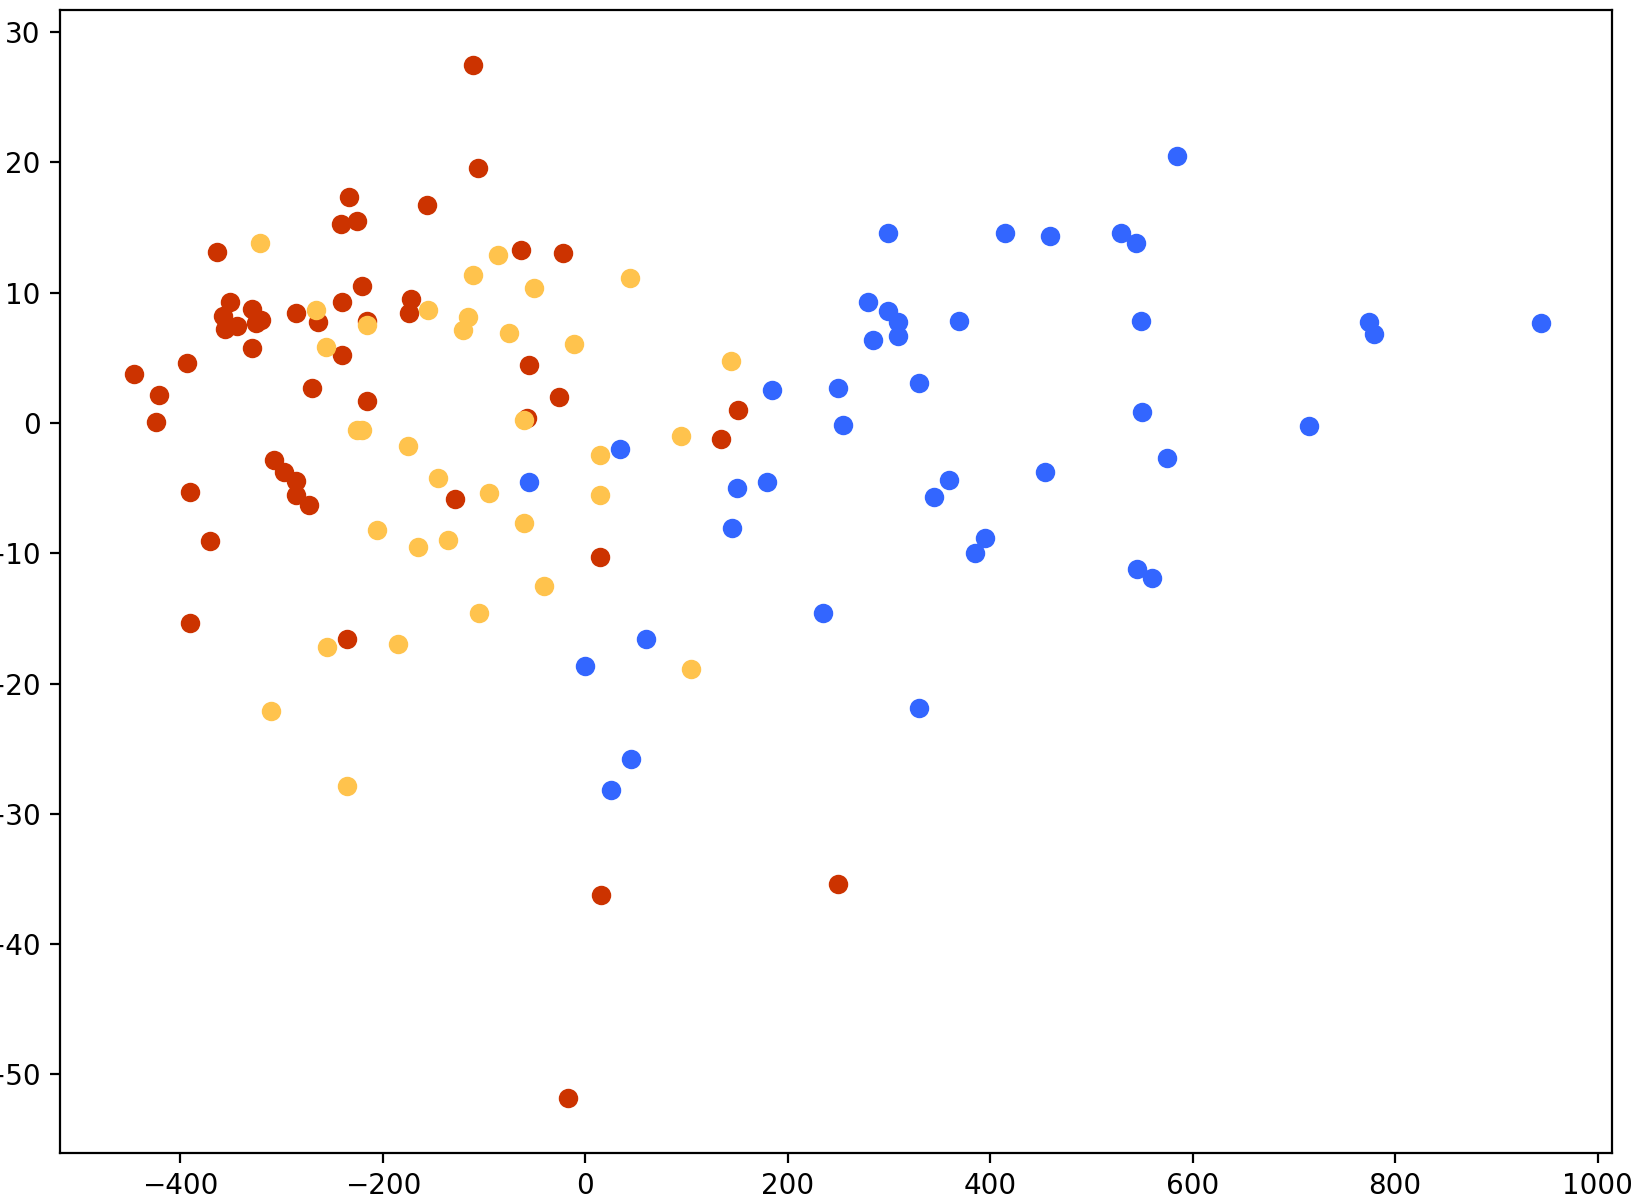
\includegraphics[height=4.2cm]{pca.png}
\caption{Fig 8: Plot of PCA-reduced train\_set}
\end{subfigure}%
\begin{subfigure}{.5\textwidth}
\centering
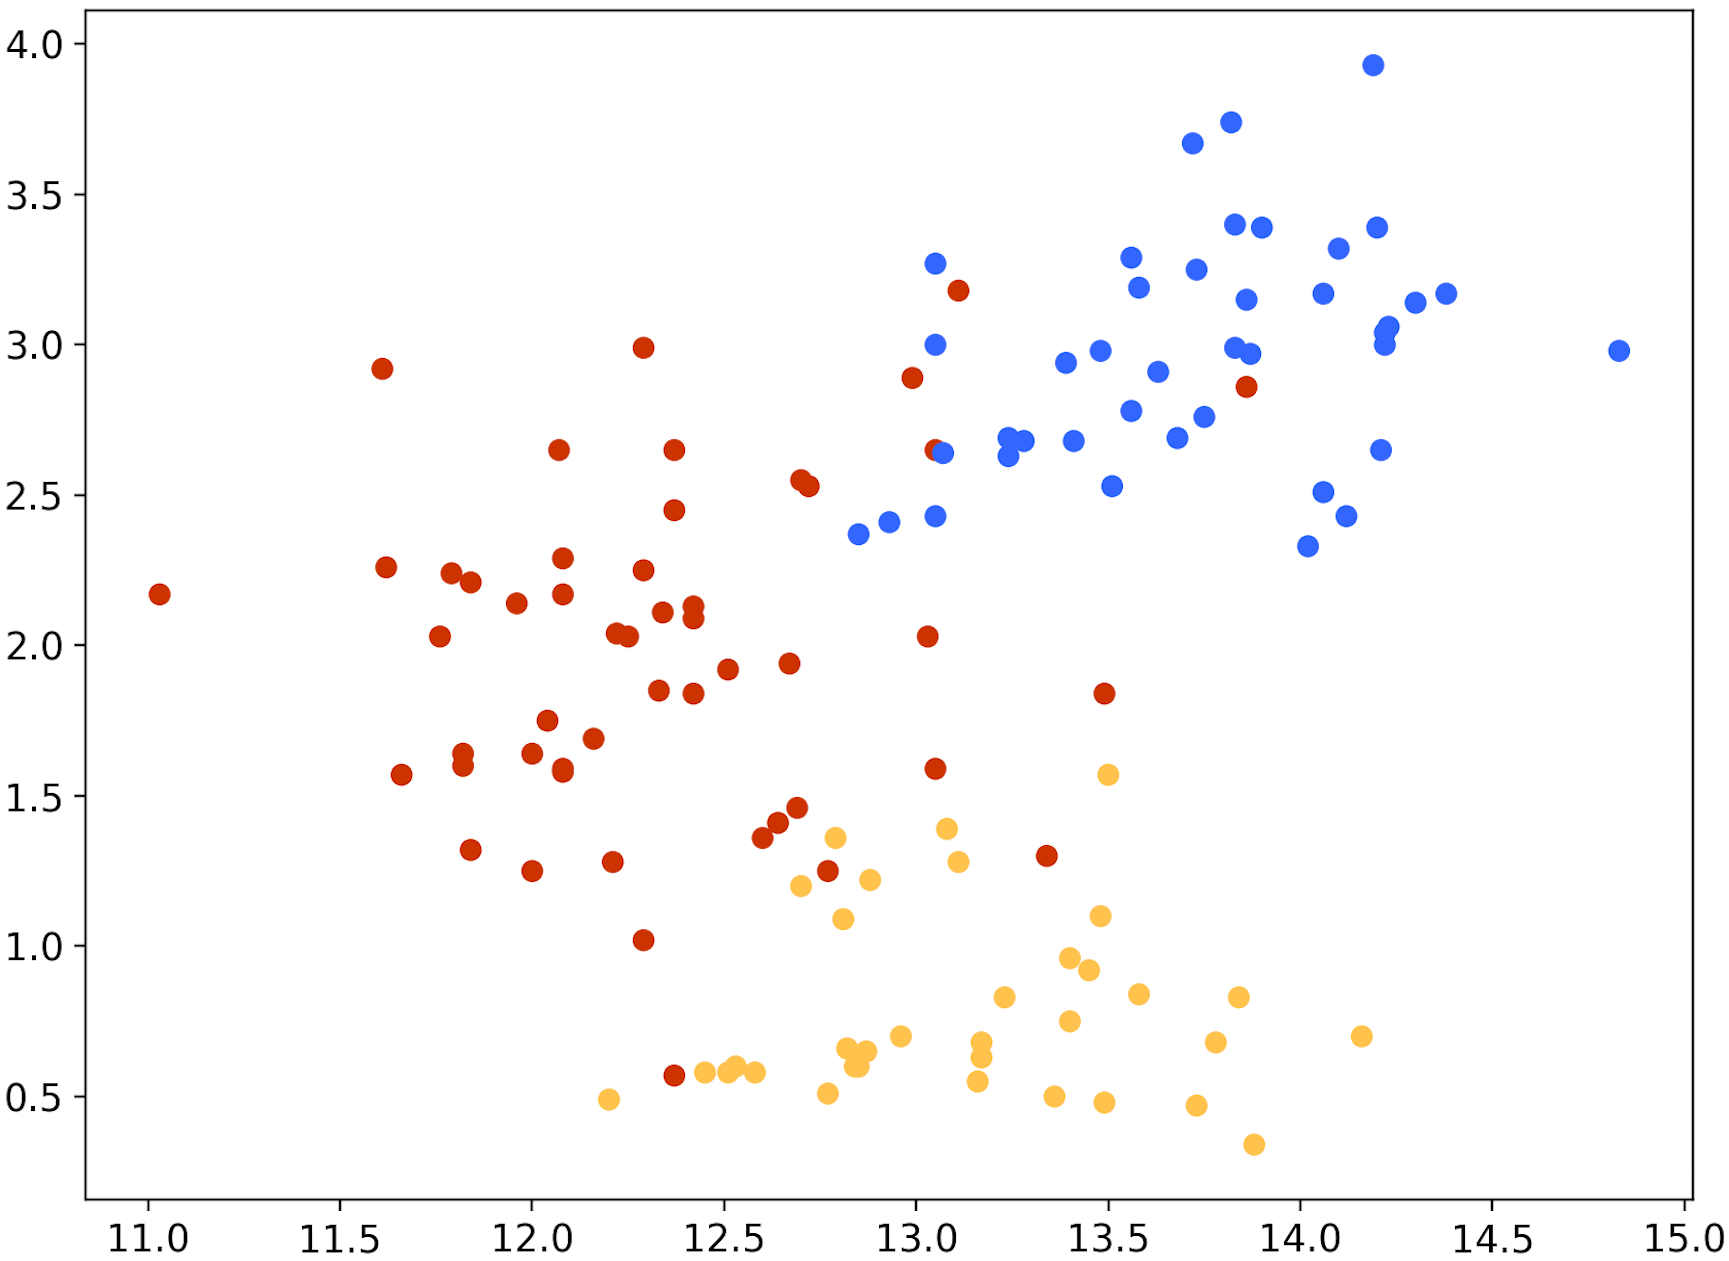
\includegraphics[height=4.2cm]{1and7.png}
\caption{Fig 9: Plot of features 1 and 7}
\end{subfigure}%
\end{figure}
\noindent

\end{document}  























